\documentclass[hidelinks,12pt]{article}
\usepackage[left=0.25cm,top=1cm,right=0.25cm,bottom=1cm]{geometry}
%\usepackage[landscape]{geometry}
\textwidth = 20cm
\hoffset = -1cm
\usepackage[utf8]{inputenc}
\usepackage[spanish,es-tabla]{babel}
\usepackage[autostyle,spanish=mexican]{csquotes}
\usepackage[tbtags]{amsmath}
\usepackage{nccmath}
\usepackage{amsthm}
\usepackage{amssymb}
\usepackage{mathrsfs}
\usepackage{graphicx}
\usepackage{subfig}
\usepackage{standalone}
\usepackage[outdir=./Imagenes/]{epstopdf}
\usepackage{siunitx}
\usepackage{physics}
\usepackage{color}
\usepackage{float}
\usepackage{hyperref}
\usepackage{multicol}
%\usepackage{milista}
\usepackage{anyfontsize}
\usepackage{anysize}
%\usepackage{enumerate}
\usepackage[shortlabels]{enumitem}
\usepackage{capt-of}
\usepackage{bm}
\usepackage{relsize}
\usepackage{placeins}
\usepackage{empheq}
\usepackage{cancel}
\usepackage{wrapfig}
\usepackage[flushleft]{threeparttable}
\usepackage{makecell}
\usepackage{fancyhdr}
\usepackage{tikz}
\usepackage{bigints}
\usepackage{scalerel}
\usepackage{pgfplots}
\usepackage{pdflscape}
\pgfplotsset{compat=1.16}
\spanishdecimal{.}
\renewcommand{\baselinestretch}{1.5} 
\renewcommand\labelenumii{\theenumi.{\arabic{enumii}})}
\newcommand{\ptilde}[1]{\ensuremath{{#1}^{\prime}}}
\newcommand{\stilde}[1]{\ensuremath{{#1}^{\prime \prime}}}
\newcommand{\ttilde}[1]{\ensuremath{{#1}^{\prime \prime \prime}}}
\newcommand{\ntilde}[2]{\ensuremath{{#1}^{(#2)}}}

\newtheorem{defi}{{\it Definición}}[section]
\newtheorem{teo}{{\it Teorema}}[section]
\newtheorem{ejemplo}{{\it Ejemplo}}[section]
\newtheorem{propiedad}{{\it Propiedad}}[section]
\newtheorem{lema}{{\it Lema}}[section]
\newtheorem{cor}{Corolario}
\newtheorem{ejer}{Ejercicio}[section]

\newlist{milista}{enumerate}{2}
\setlist[milista,1]{label=\arabic*)}
\setlist[milista,2]{label=\arabic{milistai}.\arabic*)}
\newlength{\depthofsumsign}
\setlength{\depthofsumsign}{\depthof{$\sum$}}
\newcommand{\nsum}[1][1.4]{% only for \displaystyle
    \mathop{%
        \raisebox
            {-#1\depthofsumsign+1\depthofsumsign}
            {\scalebox
                {#1}
                {$\displaystyle\sum$}%
            }
    }
}
\def\scaleint#1{\vcenter{\hbox{\scaleto[3ex]{\displaystyle\int}{#1}}}}
\def\bs{\mkern-12mu}


\title{Método de expansión en eigenfunciones  \large {Bases completas}\vspace{-3ex}}

\author{M. en C. Gustavo Contreras Mayén}
\date{ }

\pagestyle{fancy}
\fancyhf{}
\rhead{Curso MAF}
\lhead{\leftmark}
\rfoot{\thepage}
\setlength{\headheight}{16pt}%


\begin{document}
\maketitle
\fontsize{14}{14}\selectfont
\tableofcontents
\newpage

%ref. Herman (2015) 4.3 The eigenfunction expansion method
\section{Expansión en eigenfunciones.}

En este material resolveremos el problema no homogéneo $\mathcal{L} \, y = f$ usando expansiones sobre la base de las eigenfunciones de Sturm-Liouville. Hemos visto que los problemas de eigenvalores de Sturm-Liouville tienen el conjunto necesario de eigenfunciones ortogonales. En esta parte, aplicaremos el método de desarrollo de eigenfunciones para resolver un problema de valores en la frontera no homogéneo en particular.

\section{El problema no homogéneo.}

Recordemos que iniciamos con una ecuación diferencial no homogénea:
\begin{align*}
\mathcal{L} \, y = f
\end{align*}
donde $y (x)$ debe satisfacer las condiciones de frontera homogéneas dadas. El método de expansión hace uso de las eigenfunciones que satisfacen el problema de eigenvalor:
\begin{align*}
\mathcal{L} \, \phi_{n} = - \lambda_{n} \, \sigma \, \phi_{n}
\end{align*}
sujeta a las condiciones de frontera dadas. Entonces, suponemos que $y (x)$ se puede escribir como una expansión de las eigenfunciones:
\begin{align*}
y (x) = \nsum_{n=1}^{\infty} c_{n} \, \phi_{n} (x)
\end{align*}
y sustituimos la expansión en la ecuación no homogénea. Esto nos da:
\begin{align*}
f (x) = \mathcal{L} \bigg( \nsum_{n=1}^{\infty} c_{n} \, \phi_{n} (x) \bigg) = - \nsum_{n=1}^{\infty} c_{n} \, \lambda_{n} \, \phi_{n} (x)
\end{align*}
Luego, los coeficientes de expansión $c_{n}$ se calculan haciendo uso de la ortogonalidad de las eigenfunciones. Es decir, multiplicamos la última ecuación por $\psi_{m} (x)$ y posteriormente integramos, obteniendo:
\begin{align*}
\scaleint{6ex}_{\bs a}^{b} f (x) \, \phi_{m} (x) \dd{x} = - \nsum_{n=1}^{\infty} c_{n} \, \lambda_{n} \, \scaleint{6ex}_{\bs a}^{b} \phi_{n} (x) \, \phi_{m} (x) \sigma (x) \dd{x}
\end{align*}
La ortogonalidad nos lleva a:
\begin{align*}
\scaleint{6ex}_{\bs a}^{b} f (x) \, \phi_{m} (x) \dd{x} = - c_{m} \, \lambda_{m} \, \scaleint{6ex}_{\bs a}^{b} \big[ \phi_{m} (x) \big]^{2} \, \sigma (x) \dd{x}
\end{align*}
Resolviendo para $c_{m}$:
\begin{align*}
c_{m} = \dfrac{\scaleint{6ex}_{\bs a}^{b} f (x) \, \phi_{m} (x) \dd{x}}{\lambda_{m} \, \scaleint{6ex}_{\bs a}^{b} \big[ \phi_{m} (x) \big]^{2} \, \sigma (x) \dd{x}}
\end{align*}

\subsection{Ejemplo del método.}

\begin{ejemplo}
Consideremos la solución del problema del valor en la frontera:
\begin{align}
(x \, \pderivada{y})^{\prime} + \dfrac{y}{x} = \dfrac{1}{x} \hspace{1.3cm} x \in [1, e] \label{eq:ecuacion_04_24} \\
y (1) = 0 = y (e) \label{eq:ecuacion_04_25}
\end{align}
Esta ecuación ya está en forma autoadjunta. Entonces, sabemos que el problema de Sturm-Liouville de eigenvalores asociado tiene un conjunto ortogonal de eigenfunciones. Primero determinamos éste conjunto. Es decir, tenemos que resolver:
\begin{align}
(x \, \pderivada{\phi})^{\prime} + \dfrac{\phi}{x} = -\lambda \, \sigma \, \phi, \hspace{1.3cm} \phi (1) = 0 =\phi (e)
\label{eq:ecuacion_04_26}
\end{align}

Organizando los términos y multiplicando por $x$, tenemos lo siguiente:
\begin{align*}
x^{2} \, \sderivada{\phi} + x \, \pderivada{\phi} + (1 + \lambda \, \sigma \, x) \, \phi = 0
\end{align*}
Esta es casi una ecuación del tipo de Cauchy-Euler. Eligiendo la función de peso $\sigma (x) = 1 / x$, llegamos a:
\begin{align*}
x^{2} \, \sderivada{\phi} + x \, \pderivada{\phi} + (1 + \lambda ) \, \phi = 0
\end{align*}
Que fácilmente se puede resolver. La ecuación característica es:
\begin{align*}
r^{2} + (1 + \lambda) = 0
\end{align*}
Se obtienen soluciones no triviales del problema de eigenvalores que satisfacen las condiciones de frontera cuando $\lambda > -1$. Las soluciones son:
\begin{align*}
\phi_{n} (x) = A \, \sin (n \, \pi \, \ln x), \hspace{1.3cm} n = 1, 2, \ldots
\end{align*}
donde $\lambda_{n} = n^{2} \, \pi^{2} - 1$.

A menudo es útil normalizar las eigenfunciones. Esto significa que uno elige el valor de $A$ para que la norma de cada eigenfunción sea uno. Así, tenemos:
\begin{align}
\begin{aligned}[b]
1 &= \scaleint{6ex}_{\bs 1}^{e} \big[ \phi_{n} (x) \big]^{2} \, \sigma (x) \dd{x} = \\[0.5em]
&= A^{2} \, \scaleint{6ex}_{\bs 1}^{e} \sin (n \, \pi \, \ln x) \, \dfrac{1}{x} \dd{x} = \\[0.5em]
&= A^{2} \, \scaleint{6ex}_{\bs 0}^{1} \sin (n \, \pi \, y) \dd{y} = \\[0.5em]
&= \dfrac{1}{2} \, A^{2}
\end{aligned}
\label{eq:ecuacion_04_27}
\end{align}
Por lo que: $A = \sqrt{2}$. Se muestran varias de las eigenfunciones en la figura (\ref{fig:figura_04_02}).
\begin{figure}[H]
    \centering
    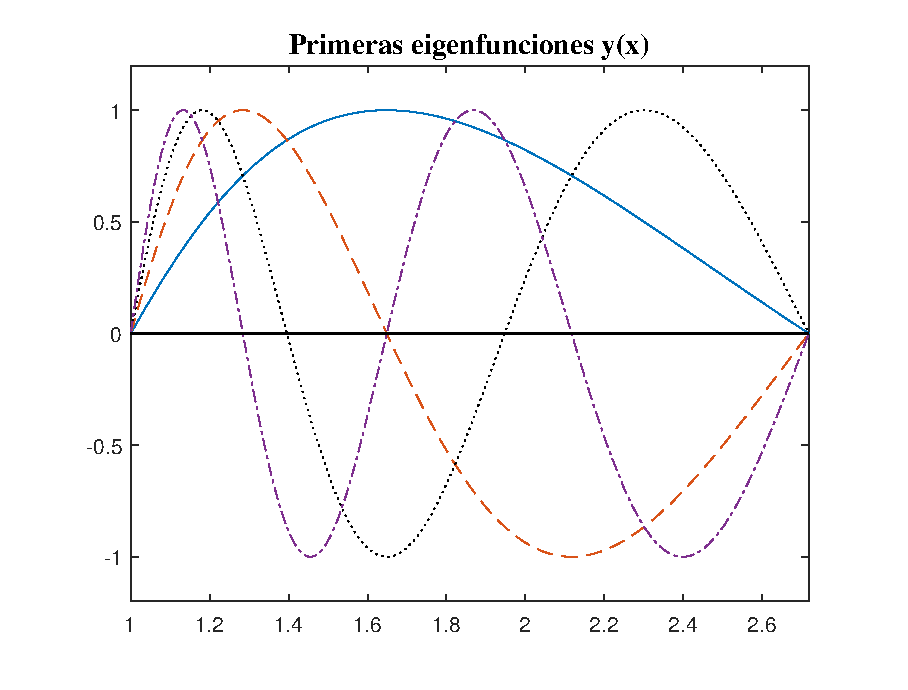
\includegraphics[scale=1]{Imagenes/Expansion_Eigenfunciones_01.eps}
    \caption{Gráfica de las eigenfunciones del ejemplo.}
    \label{fig:figura_04_02}
\end{figure}
Ahora nos enfocamos en resolver el problema no homogéneo $\mathcal{L} \, y = 1 / x$. Primero desarrollamos la solución desconocida en términos de las eigenfunciones:
\begin{align*}
y (x) = \nsum_{n=1}^{\infty} c_{n} \, \sqrt{2} (n \, \pi \, \ln x)
\end{align*}
Sustituyendo esta solución en la ecuación diferencial, se tiene lo siguiente:
\begin{align*}
\dfrac{1}{x} = \mathcal{L} \, y = - \nsum_{n=1}^{\infty} c_{n} \, \lambda_{n} \, \sqrt{2} \, \sin (n \, \pi \, \ln x) \, \dfrac{1}{x}
\end{align*}
Nuevamente usamos la ortogonalidad de las eigenfunciones. Multiplicamos ambos lados de la expresión por la eigenfunción:
\begin{align*}
\phi_{m} (x) = \sqrt{2} \, \sin (m \, \pi \, \ln x)
\end{align*}
para luego integrar, entonces tendremos que:
\begin{align*}
\lambda_{m} \, c_{m} = \scaleint{6ex}_{\bs 1}^{e} \sqrt{2} \, \sin (m \, \pi \, \ln x) \, \dfrac{1}{x} \dd{x} = \dfrac{\sqrt{2}}{m \, \pi} \, \big[ (-1)^{m} - 1 \big]
\end{align*}
Resolviendo para los $c_{m}$:
\begin{align*}
c_{m} = \dfrac{\sqrt{2}}{m \, \pi} \, \dfrac{\big[ (-1)^{m} - 1 \big]}{m^{2} \, \pi^{2} - 1}
\end{align*}
Finalmente, sustituimos estos coeficientes en la expansión de $y (x)$. La solución es entonces:
\begin{align*}
y (x) = \nsum_{n=1}^{\infty} \dfrac{2}{n \, \pi} \dfrac{\big[ (-1)^{n} - 1 \big]}{n^{2} \, \pi^{2} - 1} \sin (n \, \pi \, \ln x)
\end{align*}
La solución se muestra en la figura (\ref{fig:figura_04_03}).
\begin{figure}[H]
    \centering
    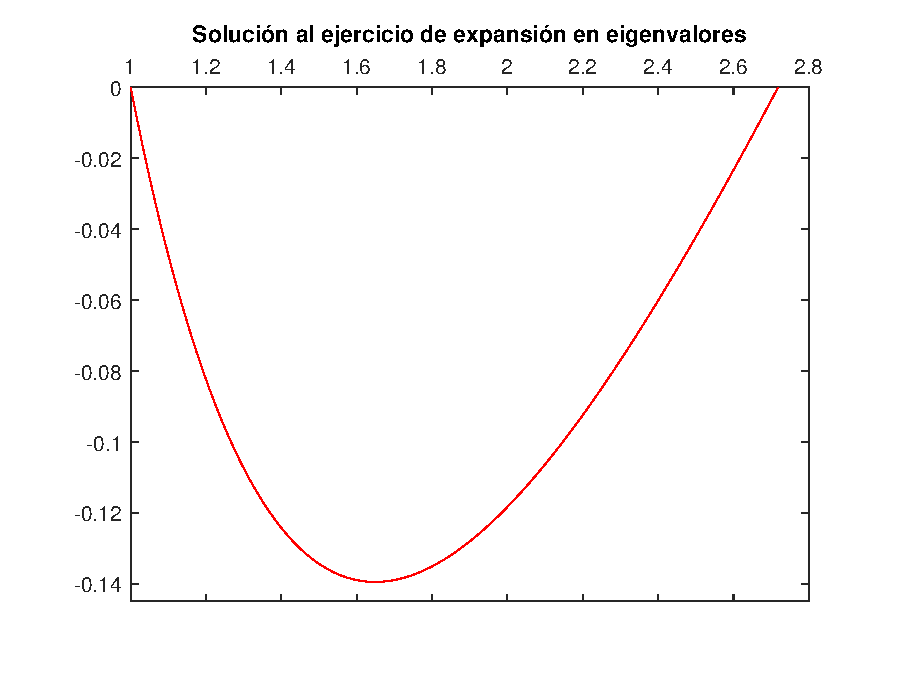
\includegraphics[scale=1]{Imagenes/Expansion_Eigenfunciones_02.eps}
    \caption{Gráfica de la solución del ejemplo, se utilizó $N = 40$.}
    \label{fig:figura_04_03}
\end{figure}
\end{ejemplo}


\end{document}